\documentclass[times, utf8, zavrsni]{fer}

\usepackage{booktabs}
\usepackage[hidelinks]{hyperref}
\usepackage{float}

\begin{document}

\thesisnumber{000}
\title{Klasifikacija uporabom umjetnih neuronskih mreža}
\author{Darijo Brčina}

\maketitle

% Ispis stranice s napomenom o umetanju izvornika rada. Uklonite naredbu \izvornik ako želite izbaciti tu stranicu.
\izvornik

% Dodavanje zahvale ili prazne stranice. Ako ne želite dodati zahvalu, naredbu ostavite radi prazne stranice.
\zahvala{}

\tableofcontents

\chapter{Uvod}
Uvod rada. Nakon uvoda dolaze poglavlja u kojima se obrađuje tema.

\chapter{Pregled područja}
Pitate li se ikada što je to inteligencija te čemu nam služi. To pitanje postavljeno je još za vrijeme začetka filozofije kao znanosti kada su se tadašnji filozofi pitali kako i na koji način je ljudsko razmišljanje, učenje i pamćenje ostvareno. Ni dan danas ne postoji jednoznačan odgovor na to pitanje jer ljudski mozak i dalje predstavlja jednu veliku nepoznanicu koja vjerojatno nikada ili ne tako skoro neće biti razriješena. No znanost je podosta napredovala i shodno tomu se razvila želja da se ljudska inteligencija pokuša pretočiti u nekakvu vrstu inteligencije strojeva.

Početak ovakvog razmišljanja datira od 50-tih godina dvadesetog stoljeća kada Alan Turing u članku \textit{Computing Machinery and Intelligence} časopisa \textit{Mind} postavlja pitanje: Mogu li strojevi misliti? \engl{Can machines think?} na koje pokušava odgovoriti kroz tzv. igru imitacije \engl{imitation game}. Sudionici igre su tri igrača: igrač A, igrač B i igrač C gdje su igrači A i B ispitanici a igrač C ispitivač. Cilj igrača C je utvrditi spol ispitanika postavljanjem pitanja, cilj igrača B je pomoći ispitivaču C a cilj igrača A je navesti ispitivača C na pogrešnu identifikaciju. Što će se dogoditi ako stroj uzme mjesto igrača A? Ako broj pogrešaka igrača C bude gotovo jednak u oba slučaja, onda je stroj inteligentan. \citep{turingAI}. Ovakav princip se često naziva turingov test \engl{Turing test}.

Nedugo nakon turingovog eksperimenta, 1956. se održava konferencija u Dartmouthu \citep{wiki:DART} na inicijativu John McCarthy-a, tadašnjeg mladog profesora matematike na fakultetu u Dartmouthu, koji okuplja oko sebe nekolicinu znanstvenika i prijatelja kako bi pokušali koncepte ljudske inteligencije preslikati u inteligenciju strojeva. Cilj je pokazati kako strojevi koriste jezik, kako zaključuju i stvaraju apstraktne koncepte i kako vremenom postaju sve prilagodljiviji na predočene probleme baš kao i ljudi. Inicijalna ideja je bila da se neki od navedenih problema može dokazati uz manju skupinu dobrih znanstvenika i kroz period od jednog ljeta (McCarthy et al. 1955). To naravno nije bilo moguće. Time se formalno uvodi pojam \textit{umjetna inteligencija}.

\section{Umjetna inteligencija}
Kao što je anticipirano ranije, umjetna inteligencija \engl{artificial intelligence} je laički rečeno inteligencija strojeva a znanost koja se jednim dijelom bavi proučavanjem umjetne inteligencije jest računarska znanost \engl{computer science}.

Primjena umjetne inteligencije danas je izrazito rasprostranjena kroz gotovo svaku industriju. Pronalazimo ju u medicini, automobilskoj industriji, robotici, pa i u sportskoj i industriji igara. Jedan od poznatijih događaja koji prikazuje primjenu umjetne inteligencije dogodio se 2016. kada je računalo naziva \textit{AlphaGo} u igri \textit{Go} uspijelo pobijediti svjetskog prvaka Lee Sedolu rezultatom 4:1 te time ostvario velik uspjeh u svijetu umjetne inteligencije kao i pažnju javnosti \citep{moyerGO}.

Umjetnu inteligenciju je dakako potrebno trenirati i učiti pa je tako učenje podijeljeno na dvije veće cjeline:
\begin{center}
    \begin{enumerate}
        \item simboličko učenje te
        \item strojno učenje.
    \end{enumerate}
\end{center}

\subsection{Simboličko učenje}
Simbolička umjetna inteligencija \engl{symbolic artificial intelligence} je izraz koji definira skup istraživačkih metoda koje se temelje na ljudima lako čitljivim simbolima \engl{human-readable simbol} koji modeliraju probleme i logiku. Jedan od najboljih primjera jesu \textit{ekspertni sustavi} koji se temelje na skupu pravila. Pravila su modelirana na sličan način kao i Ako-Onda rečenica \engl{If-Then statement} koja je u ljudskoj komunikaciji svakodnevno u upotrebi. Također, razne vrste logika poput propozicijska \engl{Propositional logic}, često referirana kao Boolova algebra, logika prvog reda \engl{First order logic}, poznatija kao predikatna logika \engl{Predicate logic}, neizrazita logika \engl{Fuzzy logic} pripadaju upravo simboličkoj umjetnoj inteligenciji. Ovakav način učenja bio je popularan početkom 1950. sve do kraja 1980 \citep{wiki:SIMB}.

\subsection{Strojno učenje}
Strojno učenje \engl{machine learning, ML} predstavlja niz metoda i algoritama koji sustavima pružaju stjecanje novog znanja kroz modeliranje obrazaca koje onda kasnije mogu iskoristiti za predviđanje novih podataka ili sličnih \citep{cupicML}. Glavna ideja je da sustavi uče iz iskustva, empirijski, bez da se programska implementacija mijenja što znatno olakšava manipulaciju istih.

Danas postoji nezgrapno puno podataka koje je moguće i koje je potrebno iskoristiti za učenje pa je cilj konstruirati sustave koji mogu iskoristiti baš te podatke za neka korisna ponašanja poput predviđanja i raspoznavanja raznih uzoraka \citep{cupicML}. Podatci se svrstavaju u dvije grupe: \textit{numerički} i \textit{kategorički} podatci. Numerički podatci su svi oni podatci nad kojima je moguće izvršiti aritmetičke operacije. Npr. unos dnevnih kalorija, broj slobodnih bacanja na košarkaškoj utakmici, isplata plaća i sl. Kategorički podatci se dodatno dijele u dvije podgrupe: nominalni i ordinalni podatci. Nominalni podatci su imenovani podatci koji nisu numerički, tj. podatci nad kojima nisu definirane aritmetičke operacije. Npr. podatci o spolu jedinke, osjećaju raspoloženja poput "tužan" ili "veseo" i sl. Ordinalni podatci također nemaju definiranu aritmetiku, no imaju definiran prirodan poredak i mogu se uspoređivati. Npr. mišljenje jedne osobe može biti "jako zadovoljan" dok druge "zadovoljan" što možemo usporediti i konstruirati prirodan poredak.

Strojno učenje dijelimo na četiri područja:
\begin{center}
    \begin{enumerate}
        \item nadzirano učenje,
        \item nenadzirano učenje,
        \item polu-nadzirano učenje te
        \item podržano učenje.
    \end{enumerate}
\end{center}

\textit{Nadzirano učenje} je tema ovog rada pa će biti obrađeno detaljnije u narednom poglavlju.

\bigskip

\textit{Nenadzirano učenje} \engl{unsupervised learning} je vrsta učenja u kojem skup podataka predstavljaju samo ulazni podatci bez znanja o tome kako bi isti trebali biti tabelirani. Zbog ovakvog pristupa, učenje je i dobilo ime nenadzirano učenje, tj. učenje bez prisustva učitelja \engl{supervisor}. Najpoznatiji postupak nenadzirano učenja je postupak grupiranja \engl{clustering}. Cilj grupiranja je na temelju danih podataka pokušati pronaći sve podatke koji imaju slična svojstva te ih zatim grupirati u odvojene razrede. Npr. neka skup ulaznih podataka sustava bude mješavina slika ljudi i slika automobila. Kao konačni rezultat, moraju se stvoriti dva razreda: razred ljudi te razred automobila. Na slici \ref{fig:clustering} prikazan je primjer grupiranja.

\begin{figure}[H]
    \centering
    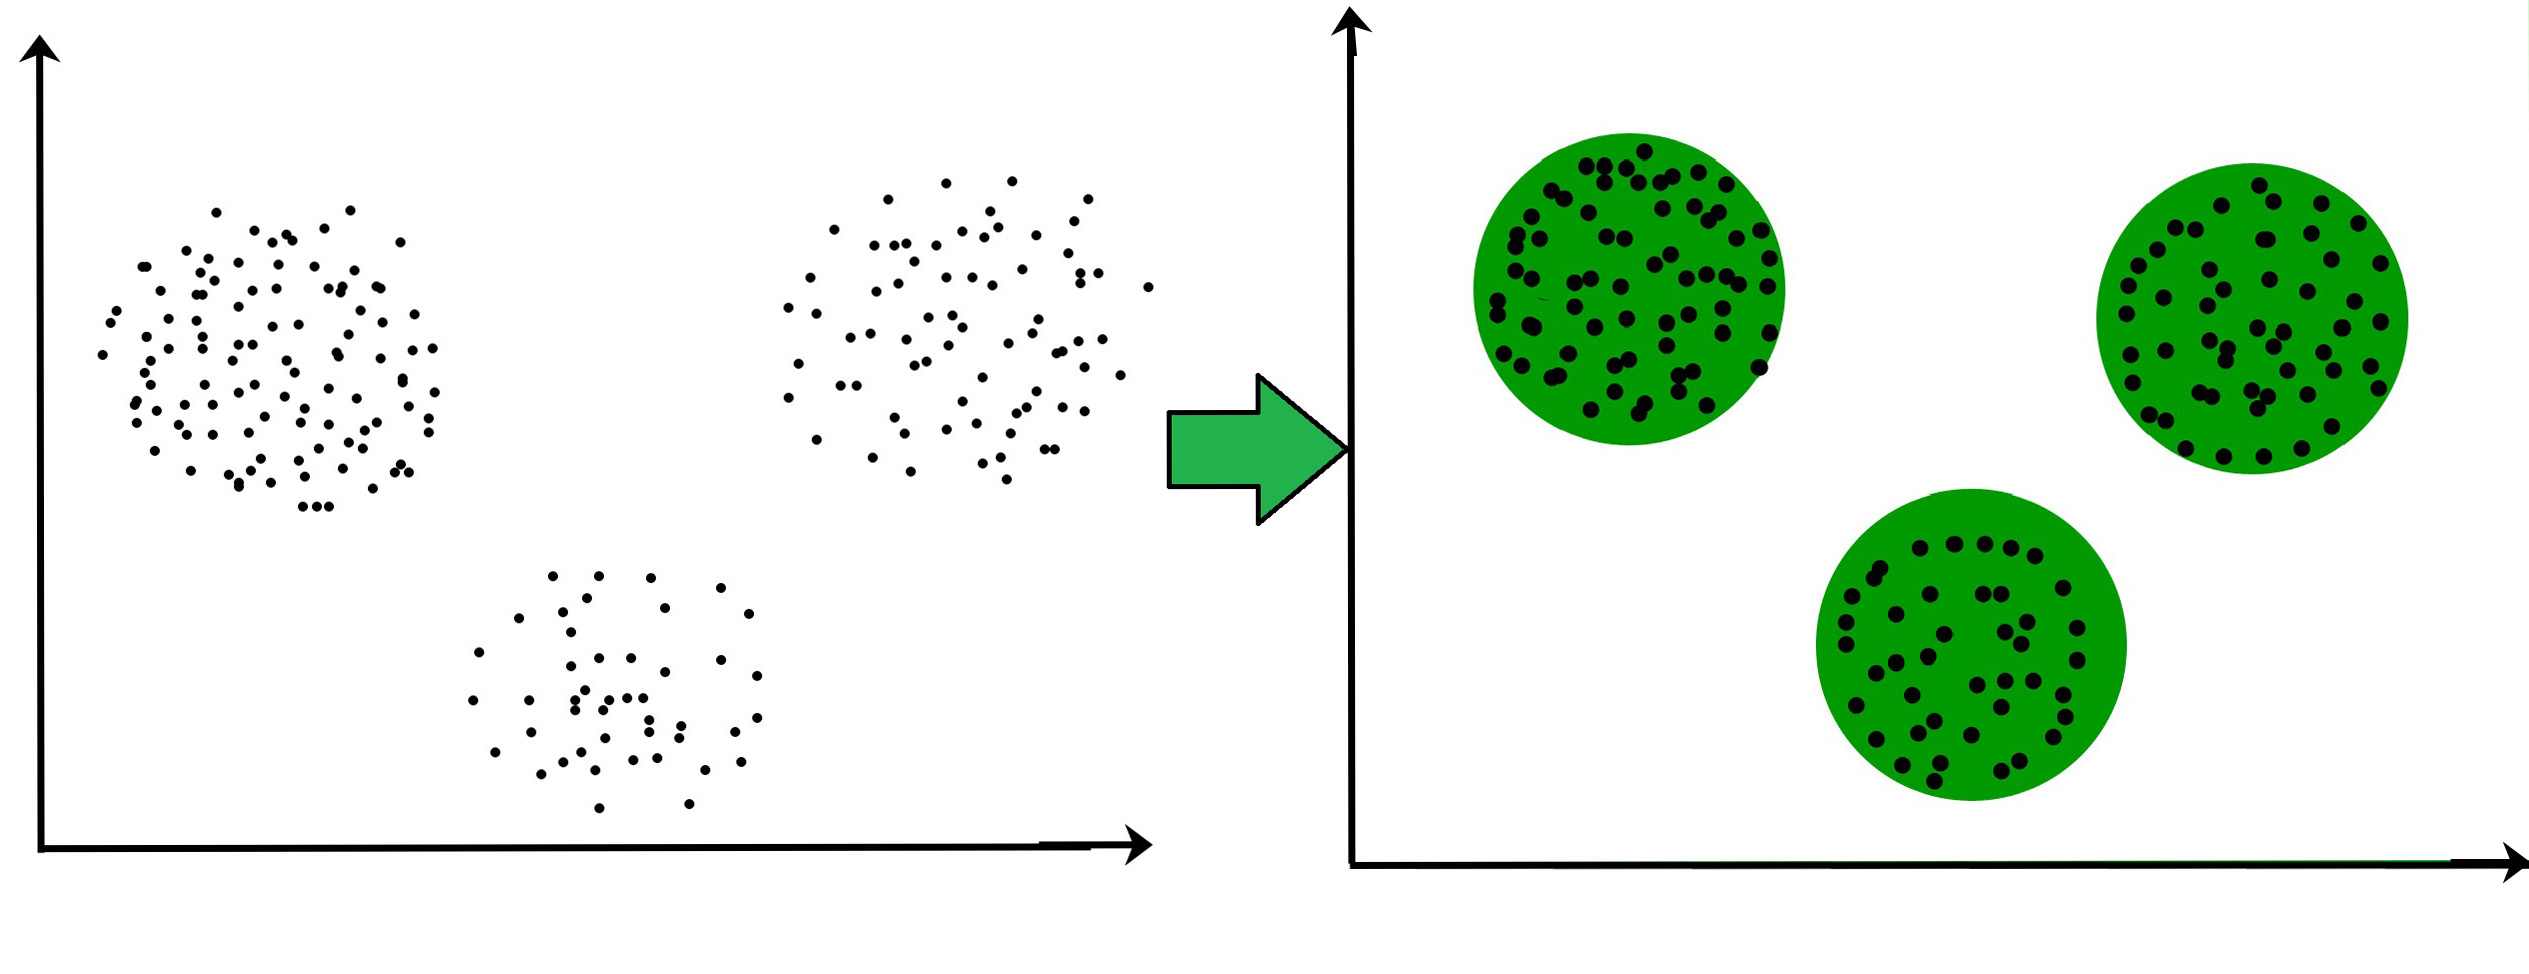
\includegraphics[scale=0.35]{img/clustering.jpg}
    \caption[Caption for LOF]{Primjer grupiranja\footnotemark}
    \label{fig:clustering}
\end{figure}
\footnotetext{Preuzeto sa https://www.geeksforgeeks.org/clustering-in-machine-learning/.}

Uz grupiranje poznati postupci su i postupci smanjenja dimenzionalnosti \engl{dimensionality reduction}, postupci otkrivanja stršećih ili novih vrijednosti \engl{outlier detection, novelty detection} i drugi.

\bigskip

\textit{Polu-nadzirano učenje} \engl{semi-supervised learning}, kao što samo ime nalaže, je učenje u kojem se isprepliću koncepti nadzirano učenje sa konceptima nenadziranim učenjem. Ono pokazuje dosta veće uspjehe nego navedeni, izvedba je izrazito zahtjevnija \citep{wiki:SEMISUP}.

\bigskip

\textit{Podržano učenje} \engl{reinforcement learning, RL} je vrsta učenja koja se potpuno razlikuje od svih do sada navedenih jer ono ne očekuje nikakve tabelirane ulazne ili izlazne podatke već je glavna ideja optimizacija ponašanja računalnih agenata. Razmatra se interakcija agenta sa okolinom \engl{environment} kroz niz akcija za koje isti može biti nagrađen ili kažnjen ovisno o ishodu akcije. Željeni cilj agenta je maksimizirati mogući dobitak nagrade \citep{wiki:RL}. Na slici \ref{fig:reinforcement-learning} prikazan je model podržanog učenja.

\begin{figure}[H]
    \centering
    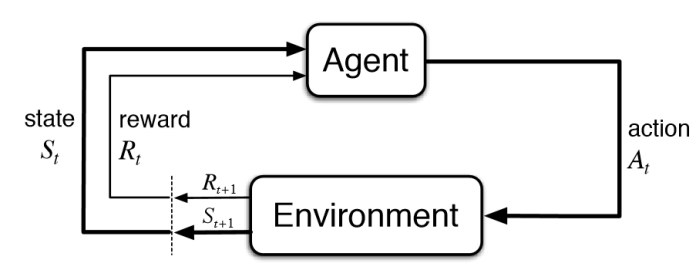
\includegraphics[scale=0.7]{img/reinforcement-learning.jpg}
    \caption[Caption for LOF]{Model podržanog učenja\footnotemark}
    \label{fig:reinforcement-learning}
\end{figure}
\footnotetext{Preuzeto sa https://www.kdnuggets.com/2018/03/5-things-reinforcement-learning.html/.}

\chapter{Nadzirano učenje}
Nadzirano učenje \engl{supervised learning} je vrsta učenja čiji je cilj sve podatke koji dođu na ulaz sustava preslikati u izlaz koji točno odgovara predanim ulazima. Dakle, prije samog učenja poznati su ulazi, koji se često modeliraju vektorima, te izlazi, koji su pridruženi tim ulazima i predstavljaju jedan podatak, stoga se tijekom učenja u svakom trenutku zna željeni izlaz te se za krive rezultate daje određena povratna informacija \engl{feedback} o tome koliko sustav griješi. Upravo zbog navedenog koncepta je učenje i dobilo ime nadzirano učenje jer se proces učenja izvršava uz prisustvo učitelja \engl{supervisor}. Razlikujemo dvije faze strojnog modela prikazane na slici \ref{fig:supervised-learning-flow}:
\begin{enumerate}
    \item faza učenja modela te
    \item faza iskorištavanja modela.
\end{enumerate}

\section{Učenje modela}

\begin{figure}[H]
    \centering
    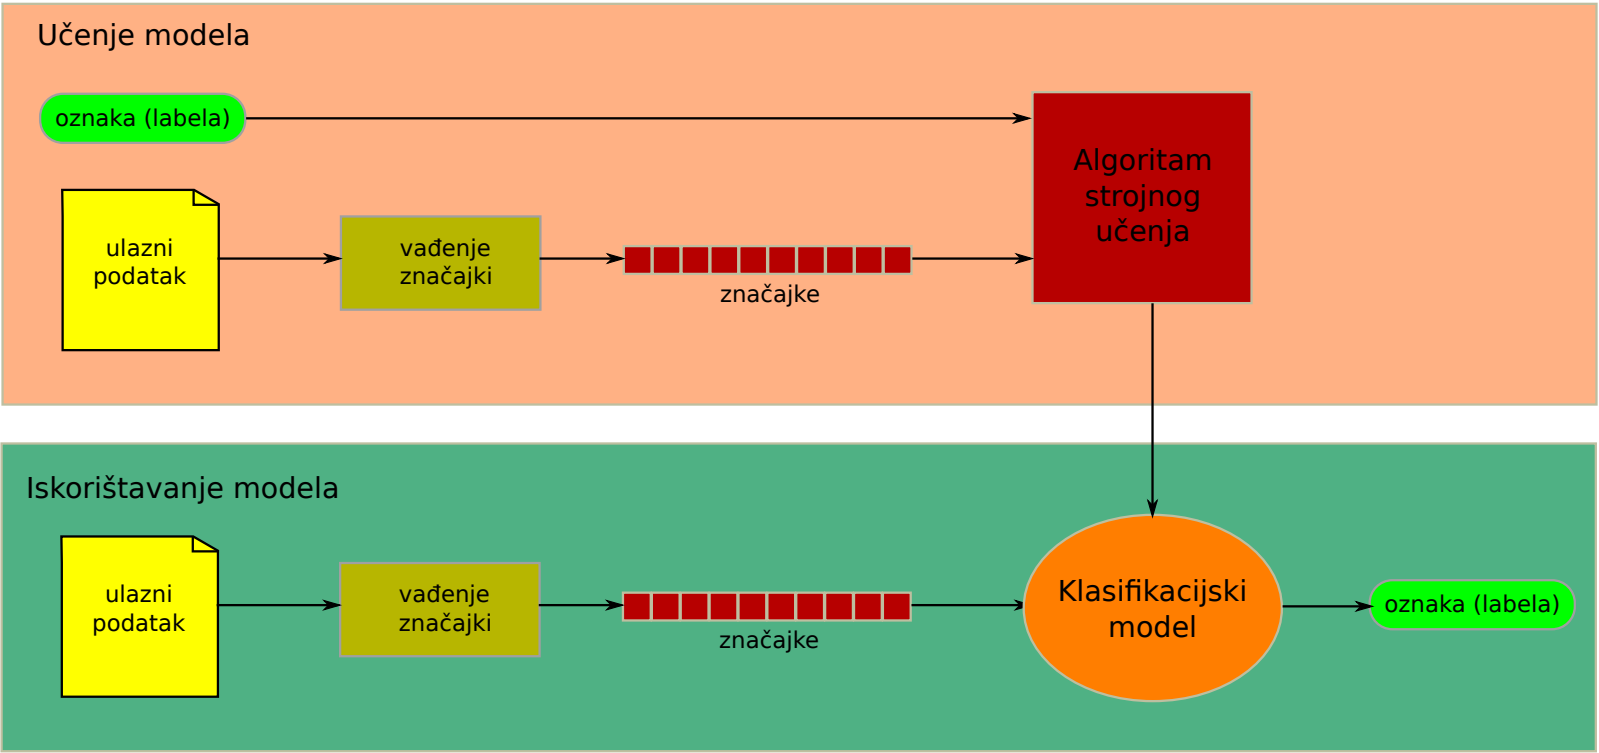
\includegraphics[scale=0.33]{img/supervised-learning-flow.png}
    \caption[Caption for LOF]{Model strojnog učenja\footnotemark}
    \label{fig:supervised-learning-flow}
\end{figure}
\footnotetext{Preuzeto iz literature \citep{cupicML}.}

Tijekom faze učenja, modelu se predaje skup ulaznih podataka za učenje \engl{training set}. Svaki podatak skupa možemo notirati kao $(\textbf{x}, y)\textsubscript{i}$ što predstavlja \textit{i}-ti testni primjer gdje \textbf{x} predstavlja vektor ulaznih podataka, a \textit{y} vrijednost pridružena ulaznom vektoru, odnosno oznaku \engl{label}. Ulazni podatak često može biti kompleksne naravi što znači da ga je potrebno "razbiti" u manje cjeline. Takav postupak se naziva vađenje značajki \engl{feature extraction}. Rezultat navedenog je kolekcija značajki koja se predaje određenom algoritmu strojnog učenja. Npr. ulazni podatci mogu biti razne gume poput gume automobila, gume bicikla, gume traktora i sl. a značajka bi onda mogla biti volumen gume, oblik gume, boja gume i sl. Algoritam strojnog učenja će na temelju predanih značajki pokušati optimizirati paremetre odabranog modela kako bi se isti mogao koristiti u sljedećoj fazi.

\bigskip

Faza iskorištavanja modela predstavlja fazu u kojoj se treba utvrditi radi li naučeni model sa podatcima nad kojima nije učio, tj. je li razvio sposobnost generalizacije \engl{generalization}. Ako model dodijeli točnu oznaku za većinu ulaznih podataka, onda možemo reći da je razvio svojstvo generalizacije. No što ako u velikoj mjeri ne uspije točno povezati izlaze sa ulazima? Ako dođe to takve pojave, kažemo da je model pretreniran \engl{overfitting}. Do navedene pojave dolazi kada model nauči previše nad skupom podataka za učenje, tj. podatke za učenje nauči savršeno raspoznavati dok za nove podatke ne uspijeva dati željene rezultate. Postoji nekoliko načina kako se može utjecati da model razvije svojstvo generalizacije a spomenut ćemo samo jedan od njih, \textit{unakrsna provjera}.

\bigskip

Unakrsna provjera \engl{cross-validation} je postupak koji se koristi tijekom faze učenja modela. Ideja je da se dio podataka iz skupa za učenje razdijeli u novi skup, skup za provjeru \engl{validation set}. Skup za provjeru često sadrži od 20\% do 30\% svih podataka iz skupa za učenje \citep{cupicML}. Tijekom faze učenja modela, model će i dalje učiti samo nad skupom za učenje dok ćemo mu povremeno dati i podatke iz skupa za provjeru čisto da se vidi koliko griješi nad njima. Važno je napomenuti da model nad podatcima iz skupa za provjeru neće učiti, tj. neće optimizirati parametre već će bit prisiljen da nauči generalizirati. Postavlja se pitanje do kada će faza učenja modela onda trajati i odgovor je vrlo jasan. Trajat će do trenutka kada pogreška nad skupom za provjeru počinje rasti. Dijagram na slici \ref{fig:cross-validation} prikazuje kako model uči kroz epohe\footnote{Epoha je ništa drugo nego jedna iteracija učenja, ali u strojnom učenju se često koristi izraz epoha pa ćemo se držati konvencije.}.

\begin{figure}[H]
    \centering
    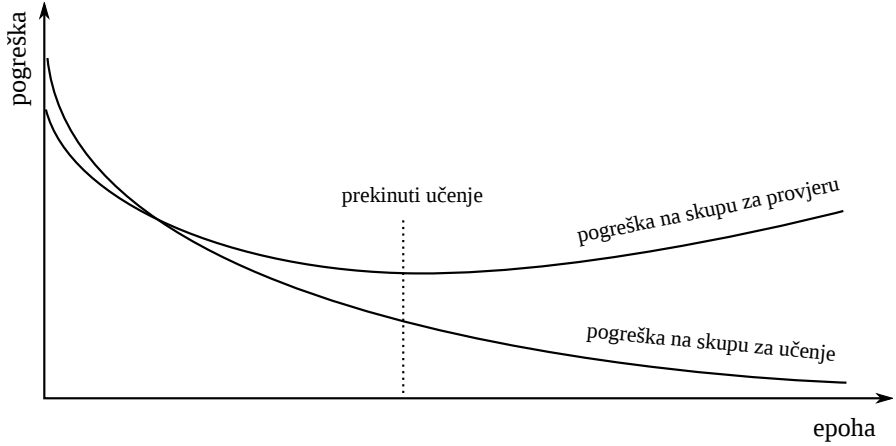
\includegraphics[scale=0.5]{img/cross-validation.png}
    \caption[Caption for LOF]{Kretanje pogrešaka pri učenju strojnog modela\footnotemark}
    \label{fig:cross-validation}
\end{figure}
\footnotetext{Preuzeto iz literature \citep{cupicANN}.}

Također postoji mogućnost da neki od parametara modela utječe na njegovu složenost. Shodno tomu se uvodi još jedan skup, skup za testiranje \engl{testing set}. Ideja je sljedeća: skup podataka razdijelimo u sva tri do sada navedena skupa i normalno provedemo fazu učenja modela uz malu promjenu. Nakon što model završi sa fazom učenja, malo ga modificiramo te ponovno učimo i sve dok ne naučimo neki određeni broj modela. Nakon što završimo sa fazom učenja onda svaki od modela ispitujemo nad skupom za testiranje te onog koji ima minimalnu pogrešku ćemo uzeti kao optimalnog \citep{cupicML}.

\section{Problemi nadziranog učenja}

Probleme koje rješavamo nadziranim učenjem su \textit{regresija} i \textit{klasifikacija}.

\subsection{Regresija}
Regresija

\subsection{Klasifikacija}
Klasifikacija

\section{Algoritmi}
Algoritmi

\chapter{Umjetne neuronske mreže}
ANN

\chapter{Rezultati}
Rezultati

\chapter{Zaključak}
Zaključak.

\bibliography{literatura}
\bibliographystyle{fer}
\nocite{*}

\begin{sazetak}
Sažetak na hrvatskom jeziku.

\kljucnerijeci{Ključne riječi, odvojene zarezima.}
\end{sazetak}

\engtitle{Classification Based on Artificial Neural Networks}
\begin{abstract}
Abstract.

\keywords{Keywords.}
\end{abstract}

\end{document}
